% *********************************************************************
% © 2016–2018 Jeremy Sylvestre
%
% Permission is granted to copy, distribute and/or modify this document
% under the terms of the GNU Free Documentation License, Version 1.3 or
% any later version published by the Free Software Foundation; with no
% Invariant Sections, no Front-Cover Texts, and no Back-Cover Texts. A
% copy of the license is included in the appendix entitled “GNU Free
% Documentation License” that appears in the output document of this
% PreTeXt source code. All trademarks™ are the registered® marks of
% their respective owners.
%
% *********************************************************************
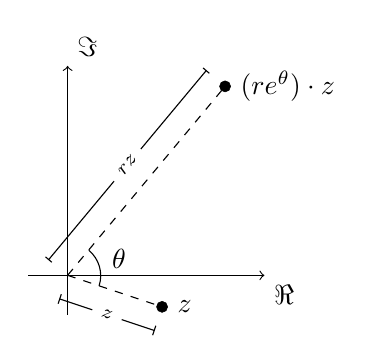
\begin{tikzpicture}[
	scale=2,
	point/.style={circle,draw,very thin,fill,inner sep=0pt,minimum size=4pt},
]
	\draw[->] (-0.25,0) to (1.25,0) node[below right] {$\Re$};
	\draw[->] (0,-0.25) to (0,1.33) node[above right] {$\Im$};

	\node[point] at (0.6,-0.2) (z) [label=right:{$z$}] {};
	\node[point] at (1,1.2) (pz) [label=right:{$(re^{\ci\theta}) \cdot z$}] {};

	\draw[dashed] (0,0) -- (z);
	\draw[dashed] (0,0) -- (pz);

	\draw (0.2,-0.067) arc (-18:50.2:0.21cm) node[midway,xshift=0.25cm,yshift=0.1cm] {$\theta$};

	% shift orthogonally from (0.3,-0.1) along (-0.2,-0.6) by (-0.05,-0.15)
	\node[rotate=-18] at (0.25,-0.25) (r) {$\scriptstyle\cmodulus{z}$};
	\draw (-0.05,-0.15) -- (r) -- (0.55,-0.35);
	\draw (-0.04,-0.12) -- (-0.06,-0.18);
	\draw (0.56,-0.32) -- (0.54,-0.38);

	% shift orthogonally from (0.5,0.6) along (-1.2,1) by (-0.12,0.1)
	\node[rotate=50.2] at (0.38,0.7) (r) {$\scriptstyle r\cmodulus{z}$};
	\draw (-0.12,0.1) -- (r) -- (0.88,1.3);
	\draw (-0.14,0.117) -- (-0.1,0.083);
	\draw (0.86,1.317) -- (0.9,1.283);

\end{tikzpicture}
